\section*{Part II -- First Concepts}
\addcontentsline{toc}{section}{Part II -- First Concepts}

\section{First Concepts: Continua, Nesting, and K-Levels}
\label{sec:r008-first-concepts-k-primer}

A continuum in OC is not merely a smooth line, an interval, or a physical
medium. It is a structured system whose admissible states, internal axes,
flows, thresholds, cycles, and boundaries allow it to persist as one thing while
changing. This definition is deliberately broad, but it is not empty. A pile of
unrelated parts is not yet a continuum. A continuum must have a state space
\(\Omega(K)\), a boundary \(\partial\Omega(K)\), structural differences
\(A(K)\), sustaining or destructive flows \(J(t)\), thresholds \(\Theta(K)\),
cycles \(C(K)\), and a continuumness measure \(k(K,t)\).

The simplest reader-facing formula is:
\[
K=\bigl(\Omega,\partial\Omega,A,\Theta,P,J,C,k,M\bigr).
\]
The tuple says that a continuum is not just what it is made of. It is also the
space of admissible states, the boundary of that space, the dimensions along
which it can vary, the thresholds that change its regime, the potentials and
flows that move it, the cycles that sustain it, the continuumness that measures
its live coherence, and the embedding context in which it can become part of
something larger.

\subsection{Continua Contain Continua}

The most important first intuition is nesting. Continua are composed of
continua and can themselves become components of larger continua. A cell
contains molecular and metabolic continua. An organism contains cellular,
neural, immunological, behavioral, and ecological continua. An enterprise
contains technical platforms, teams, processes, contracts, security controls,
knowledge flows, and markets. A scientific theory contains definitions,
models, proof routes, examples, literature relations, and research programs.

This nesting is not one linear chain for the whole world. It is closer to a
fractal matryoshka of systems. A higher level is formed from lower-level
continua and their configurations, but it is not reducible to a mere list of
parts. The configuration determines new constraints, new possibilities, and new
criticism routes. Conversely, a higher-level continuum constrains what its
lower-level continua can do. In an enterprise, an individual service can be
technically healthy and still become organizationally dead if governance,
security, economics, or user trust remove it from the admissible state space of
the enterprise.

\subsection{Why the Letter K}

The letter \(K\) is used for levels because it echoes the German word
\emph{Kontinuum}. The letter \(C\) is already heavily overloaded in many
mathematical, computational, and systems contexts, including categories,
constants, cycles, classes, and complexity. The notation \(K_x\) therefore
names a continuum level while keeping the symbols \(C(K)\) and related
families available for cycles and other structures.

\subsection{K-Levels Are Not a Mere Classification}

A K-level is not a label pasted onto a system after inspection. It is a way of
asking what kind of continuum is being formed, what lower continua compose it,
what new axis or configuration appears, what space of possibilities is opened,
and what boundary or criticism route becomes visible. The lower levels shape the
possible upper levels; the upper levels reorganize the meaning and operation of
the lower levels.

\begin{table}[htbp]
\centering
\small
\begin{tabular}{p{0.18\textwidth}p{0.35\textwidth}p{0.35\textwidth}}
\toprule
Level route & Reader question & Enterprise or AI-system analogy\\
\midrule
\(K_0\)--\(K_1\) & What minimal structure and first admissible axis exist? & A primitive data object or interface becomes addressable.\\
\(K_2\)--\(K_4\) & What physical, chemical, or protocellular constraints make stable operation possible? & Infrastructure, energy, hardware, deployment substrate, and runtime constraints become non-optional.\\
\(K_5\)--\(K_6\) & What signalling, memory, representation, or decision loop appears? & Monitoring, feedback, model state, policy memory, and agent reasoning begin to matter.\\
\(K_7\)--\(K_8\) & What social, institutional, or civilizational coordination contains the system? & Teams, governance, trust, regulation, markets, and organizational resilience constrain technical design.\\
\(K_9\)--\(K_{12}\) & What theory, formal system, meta-theory, or cross-domain synthesis governs interpretation? & Architecture doctrine, verification regime, enterprise ontology, and strategic model comparison determine how claims are judged.\\
\bottomrule
\end{tabular}
\caption{A first reader-facing interpretation of K-levels. The table is not a final proof of the hierarchy; it gives a practical entry point before the formal K0--K12 chapters.}
\label{tab:r008-k-primer}
\end{table}

% R008_K_LEVELS_PRESENT: K0 K1 K2 K3 K4 K5 K6 K7 K8 K9 K10 K11 K12.
\begin{figure}[!htbp]
\centering
\resizebox{0.98\textwidth}{!}{%
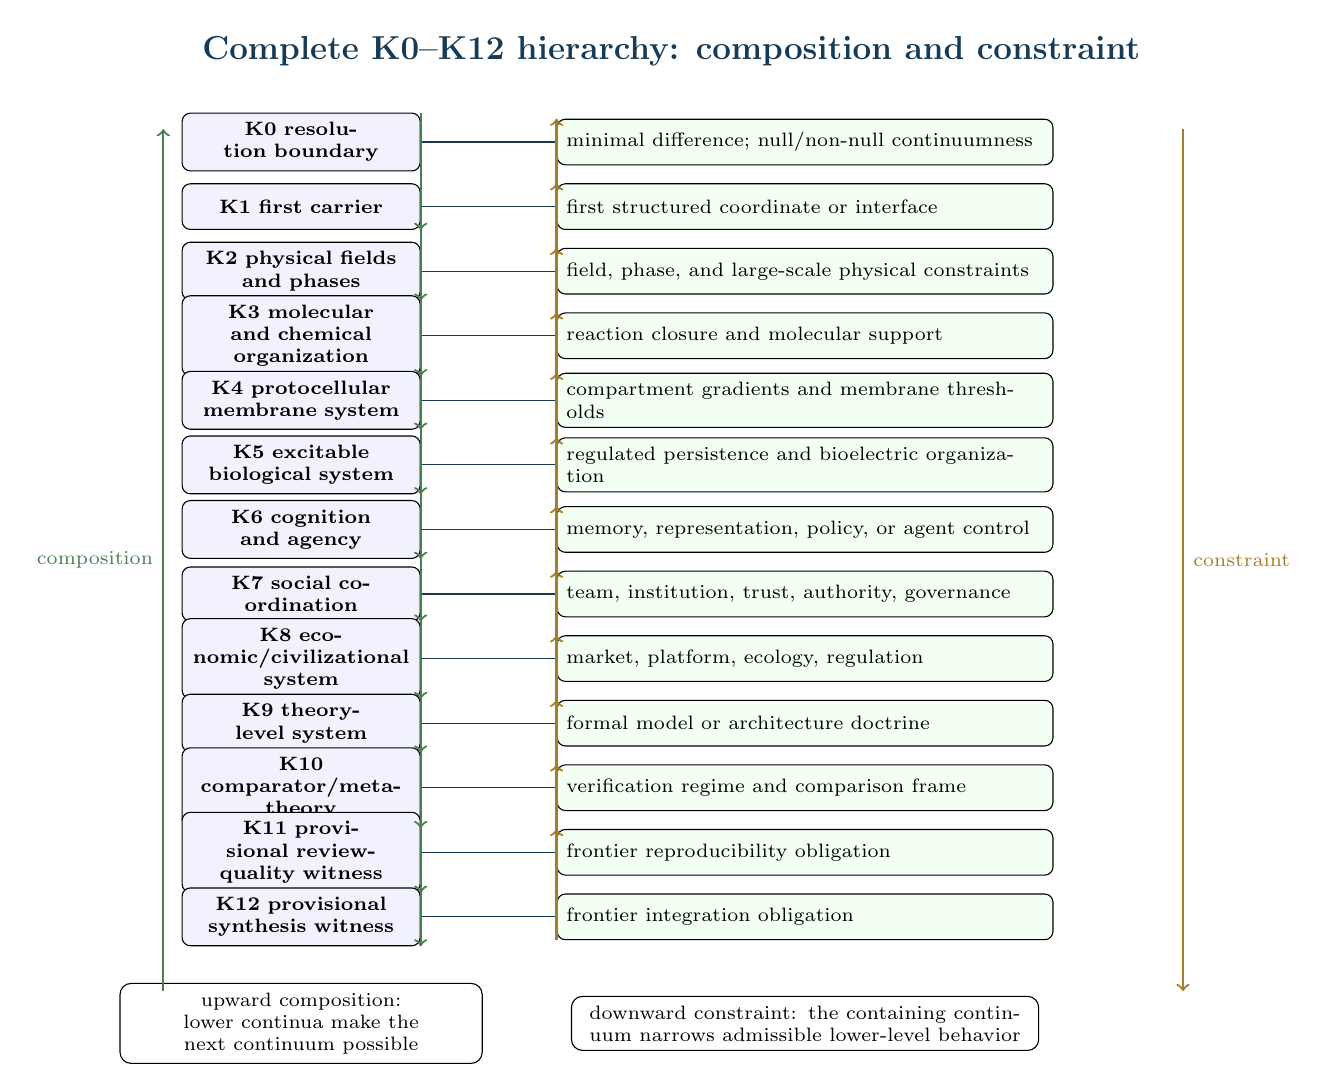
\begin{tikzpicture}[x=1cm,y=0.82cm, every node/.style={font=\scriptsize}]
  \definecolor{ocBlue}{HTML}{173B57}
  \definecolor{ocGold}{HTML}{A77D2A}
  \definecolor{ocGreen}{HTML}{4B7F52}
  \node[font=\bfseries\large, ocBlue] at (0,14.4) {Complete K0--K12 hierarchy: composition and constraint};
  \foreach \i/\human/\role in {
    0/{K0 resolution boundary}/{minimal difference; null/non-null continuumness},
    1/{K1 first carrier}/{first structured coordinate or interface},
    2/{K2 physical fields and phases}/{field, phase, and large-scale physical constraints},
    3/{K3 molecular and chemical organization}/{reaction closure and molecular support},
    4/{K4 protocellular membrane system}/{compartment gradients and membrane thresholds},
    5/{K5 excitable biological system}/{regulated persistence and bioelectric organization},
    6/{K6 cognition and agency}/{memory, representation, policy, or agent control},
    7/{K7 social coordination}/{team, institution, trust, authority, governance},
    8/{K8 economic/civilizational system}/{market, platform, ecology, regulation},
    9/{K9 theory-level system}/{formal model or architecture doctrine},
    10/{K10 comparator/meta-theory}/{verification regime and comparison frame},
    11/{K11 provisional review-quality witness}/{frontier reproducibility obligation},
    12/{K12 provisional synthesis witness}/{frontier integration obligation}
  }{
    \pgfmathsetmacro{\y}{13-\i}
    \node[draw, rounded corners=3pt, fill=blue!5, text width=0.23\textwidth, align=center, minimum height=0.58cm] (k\i) at (-4.7,\y) {\textbf{\human}};
    \node[draw, rounded corners=3pt, fill=green!5, text width=0.50\textwidth, align=left, minimum height=0.58cm] (r\i) at (1.7,\y) {\role};
    \draw[-, ocBlue] (k\i.east) -- (r\i.west);
  }
  \foreach \i in {0,...,11}{
    \pgfmathtruncatemacro{\j}{\i+1}
    \draw[->, ocGreen, line width=0.8pt] (k\i.north east) -- (k\j.south east);
    \draw[->, ocGold, line width=0.8pt] (r\j.south west) -- (r\i.north west);
  }
  \node[draw, rounded corners=4pt, fill=white, text width=0.36\textwidth, align=center] at (-4.7,-0.65)
    {upward composition: lower continua make the next continuum possible};
  \node[draw, rounded corners=4pt, fill=white, text width=0.47\textwidth, align=center] at (1.7,-0.65)
    {downward constraint: the containing continuum narrows admissible lower-level behavior};
  \draw[->, thick, ocGreen] (-6.45,-0.15) -- (-6.45,13.2) node[midway,left,align=center] {composition};
  \draw[->, thick, ocGold] (6.5,13.2) -- (6.5,-0.15) node[midway,right,align=center] {constraint};
\end{tikzpicture}}
\caption{The full K-level teaching ladder. The figure does not merely decorate the text: it demonstrates the two central dependencies used later in the formal hierarchy. Every K0--K12 level is numbered and named; the left column shows composition upward, and the right column shows how a higher continuum constrains its parts.}
\label{fig:r008-k0-k12-hierarchy}
\end{figure}

\subsection{What Characterizes a K-Level}

Each K-level is characterized by at least five questions. First, what lower
continua are required? Second, what new axis or configuration appears? Third,
what admissible state space becomes possible? Fourth, what cycles or flows
sustain the new level? Fifth, what boundary or death condition would collapse
it? These questions keep the hierarchy operational. A level is not accepted
because it sounds plausible; it must name the structural difference that earns
its place.

\subsection{A Practical Enterprise Example}

Consider an AI-enabled enterprise risk system. At one level, there are compute
resources, networks, storage, and data pipelines. At another level, there are
models, embeddings, prompts, policies, and evaluation traces. At a higher
level, there are teams, approvals, legal obligations, customer trust, business
strategy, and public reputation. A failure in one layer can move another layer
outside its admissible state space: a model update can break compliance, a
security event can collapse trust, a governance delay can make an otherwise
correct technical system operationally unusable. OC gives this situation a
single structural vocabulary without pretending that infrastructure, law,
economics, and cognition are the same discipline.

\subsection{How the Primer Leads into the Formal Core}

The next parts of the monograph make this intuition exact. The formal core
defines state spaces, boundaries, thresholds, potentials, flows, cycles,
continuumness, operators, and K-level witnesses. The evidence parts then ask
which of those claims are supported by proof, finite semantics, replay QA,
numeric rows, comparator analysis, and falsifier tests. The reader should now
have the map: continua contain continua, K-levels name structured emergence,
and the rest of the manuscript tests how far that grammar can be made precise.


% R008_FIGURE_SPEC_VALIDATED: K0-K12 labels, composition arrows, constraint arrows, semantic role text, and non-overlap layout.
